\chapter{Protezione Microdati}
\label{microdata_protection}

\section{Introduzione}

\section{Macrodata vs Microdata}

\section{Classificazione delle tecniche di protezione riguardo il Disclosure dei microdati}
Il controllo del disclosure dei microdati è un’importante problema pratico sia nel privato che nel pubblico.
$\\$
La protezione dei microdati ha apparentemente due obiettivi tra di loro contrastanti. Da una parte si vuole evitare la re-identificazione, la quale accade ogni qualvolta l’informazione del respondent che appare nella table di microdati è identificata; il quale, è associata con le identità dei respondent corrispondenti.
$\\$
Dall’altra invece le applicazioni di tecniche dovrebbero preservare le *chiavi delle proprietà statistiche* dei dati originali i quali sono state segnati come importanti dai destinatari dei dati (ossia chi riceverà i dati finali)

$\\$
Precisamente data una table di microdati T, una tecnica di protezione dei dati dovrebbe trasformare questa table T in una table $T_1$ in modo che:
\begin{enumerate}
    \item il rischio che un utente malevolo possa usare $T_1$ per determinare informazioni confidenziali o identificare un respondent, sia basso
    \item l’analisi statistica su T e $T_1$ possa produrre risultati simili
\end{enumerate}

Generalmente i seguenti fattori contribuiscono al rischio di disclosure:

\begin{itemize}
    \item L’esistenza di tuple altamente visibili (ossia tutte quelle tuple con caratteristiche che hanno caratteristiche uniche)
    \item Possibilità di matching tra le table di microdati e le informazioni esterne.
    \item L’esistenza di un alto numero degli attributi comuni che possono aumentare la possibilità di linking.
\end{itemize}

Mentre i fattori che minimizzano il rischio di disclosure sono:
\begin{itemize}
    \item Una table di microdati contenenti un subset della popolazione intera.
    Questo implica che le informazioni di un respondent specifico, il quale potrebbe essere un utente malevolo potrebbe voler sapere, potrebbe non essere incluso nella table di microdati.
    \item Le informazioni specificate nelle table rilasciate, quindi pubbiche non sono aggiormate. Potrebbero cambiare nel tempo, indi per cui il linking con le informazioni esterne potrebbero non essere accurati
    \item Una table di microdati e le informazioni esterne contengono rumore, riducendo la probabilità di linking delle informazioni
    \item Una table di microdati e le risorse esterne possono contenere dati espressi in forme diverse, riducendo l’abilità di linking
\end{itemize}

\begin{figure}[h]
    \centering
    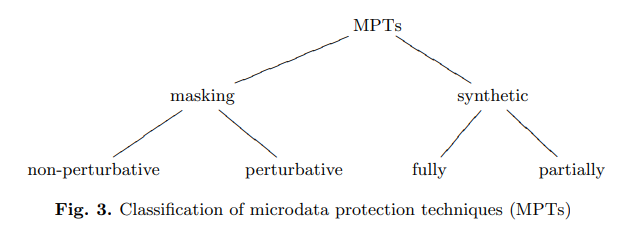
\includegraphics[width=0.5\linewidth]{paper_microdata/Fig3.png}
    \caption{Classificazione delle tecniche di protezione dei microdati}
    \label{fig:Fig 3}
\end{figure}

$\\$
Generalmente, per limitare il rischio di disclosure di una table di microdati è necessario sopprimere gli identifiers impliciti ed espliciti come step iniziale (e.g. SSN, Name)

$\\$
Questo processo  è noto come de-identificazione, quest’ultima non necessariamente rende le tuple anonime, siccome è possibile fare re-identificazione usando informazioni esterne.

$\\$
Tipicamente le tecniche sono basate sul principio che la re-identificazione possa essere contrastata riducendo la quantità delle informazioni rilasciate, mascherando i dati (e.g., non rilasciando o perturbando i valori), o rilasciando valori plausibili modificati invece di quelli reali. Seguendo questo principio le tecniche si suddividono in duo macro categorie: 
\begin{itemize}
    \item Tecniche di mascheramento: I dati originali sono trasformati producendo nuovi dati che non sono validi per le analisi statistiche in modo da preservare la confidenzialità dei respondent. Le tecniche di mascheramento si suddividono in:
    \begin{itemize}
        \item non perturbative: il dato originale non viene modificato, ma alcuni dati vengono soppressi o vengono rimossi dettagli.
        \item perturbativi: i dati originali sono modificati.
    \end{itemize}
    \item Generazione dei dati sintetici: I set di tuple originale nelle table di microdati sono sostituiti da un nuovo set di tuple generati in modo di preservare le proprietà statistiche chiave del dato originale.% Il processo di generazione è basato sui modelli statistici e le proprietà statistiche delle chiavi che non sono incluse nei modelli%
    Dal momento che le table dei microdati rilasciati contengono dati sintetici, il rischio di re-identificazione viene ridotto.
    Questi possono essere interamente sintetici (fully synthetic) o misti con i dati originali (partially synthetic).

    $\\$
    Un'altra caratteristica importante delle tecniche di protezione è che possono essere usati su tipo di dati differenti. In particolare i tipi di dati possono essere categorizzati come 
    \begin{itemize}
        \item \textit{Continui}: Un attributi è detto continuo se le operazioni numeriche e aritmetiche sono definite sull'attributo. E.g. Data di nascita e temperatura sono attributi continui.
        \item \textit{Categorici}: Un attributo è definito categorico se le operazioni aritmetiche non hanno alcun senso se fatto sull'attributo. E.g. Razza, su cui non si possono fare operazioni aritmetiche
    \end{itemize}
\end{itemize}
$\\$
Di seguito, sono descritti le tecniche di protezione dei microdati principali, e se sono applicabili a dati continui, categorici o entrambi.
\begin{figure}[h]
    \centering
    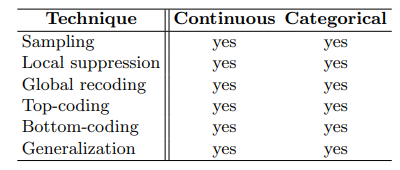
\includegraphics[width=0.5\linewidth]{paper_microdata/Fig4.png}
    \caption{Applicazione delle tecniche non perturbative su dati differenti}
    \label{fig:Fig-4}
\end{figure}

\begin{figure}[h]
    \centering
    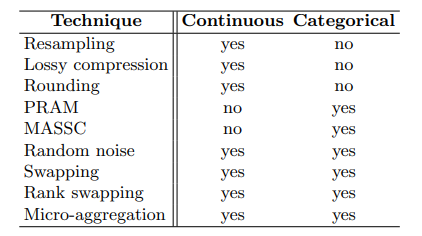
\includegraphics[width=0.5\linewidth]{paper_microdata/Fig5.png}
    \caption{Applicazione delle tecniche perturbative su dati differenti}
    \label{fig:Fig-5}
\end{figure}

\section{Tecniche di Mascheramento}
Alcune tecniche di mascheramento

\subsection{Tecniche non perturbative}
Le tecniche non perturbative producono microdati eliminando dettagli dai dati originali. Di seguito alcune di esse:

\begin{itemize}
    \item \textit{Sampling}: I table dei microdati protetti includono solo tuple formate da sample (campioni) della popolazione totale. Siccome c'è dell'incertezza se uno specifico respondent sia presente nei sample, il rischio di re-identificazione viene riudotto. Per esempio possiamo decidere se pubblicare solo le tuple pari della table originale. Questa tecnica può operare solo su dati categorici 
    
    \item \textit{Local suppression}: Sopprime i valori degli attributi in modo da limitare la possibilità di analisi. Questa tecnica lascia uno spazio vuoto su alcuni attributi (sensitive cells) che contribuiscono in modo significante al rischio di disclosure delle tuple coinvolte.
    
    \item \textit{Global Recoding}: Il dominio degli attributi, ossia tutti i possibili valori, sono divisi intervalli disgiunti di grandezza uguale, e ogni intervallo viene associato a una label. La table dei microdati protetti sono ottenuti sostituendo i valori degli attributi con le label associate agli intervalli corrispondenti. Questa tecnica riduce i dettagli della table e quindi riduce il rischio di re-identificazione. Sono presenti due tecniche particolari di recoding, ossia \textit{Top-Coding} e \textit{Bottom-Coding}, qui sotto descritte:
    \begin{itemize}
        \item \textit{Top-Coding}: E' basata sulla definizione di limite superiore (upper limit), chiamato top-code, per ogni attributo che deve essere protetto. Ogni valore maggiore di questo valore è sostituito dal top-code. Questa tecniche può essere applicata agli attributi categorici che possono essere ordinati linearmente come gli attributi continui.  
        \item \textit{Bottom-Coding}: Simile al top-coding ma definisce il limite inferiore (lower limit). Quindi, ogni valore più basso di questo non verrà ripubblicato e verrà sostituito con il bottom-code.
    \end{itemize}
    \item \textit{Generalization}: Consiste nel rappresentare i vaori di un dato attributo usando valori più generali. Questa tecnica è basata sulla definizione di generalizzazione gerarchica, dove i valori più generali sono alla radice della gerarchia e le foglie corrispondono ai valori specifici. Un processo di generalizzazione perciò procede con la sostituzione dei valori rappresentati dai nodi foglia con dei valori al nodo superiore.

    \begin{figure}[h]
        \centering
        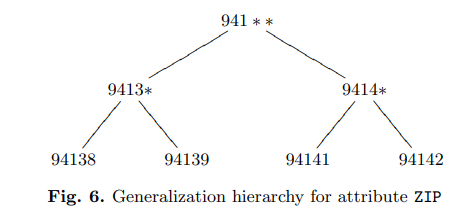
\includegraphics[width=0.5\linewidth]{paper_microdata/Fig6.png}
        \caption{Generalizzazione gerarchica}
        \label{fig:Fig-6}
    \end{figure}
\end{itemize}

\subsection{Tecniche perturbative}
Con le tecniche perturbative le table dei microdati vengono modificate per la pubblicazione
Le modifiche possono portare a combinazioni dei valori originali uniche le quali svaniscono non appena vengono introdotte nuove combinazioni.
\begin{itemize}
    \item \textit{Resampling}: Questa tecnica sostituisce i valori degli attributi sensibili continui con un valore medio computato sul numero di samples della popolazione originaria. Precisamente, assumiamo che $N$ sia il numero di tuple presenti in una table di microdati, e $S_1,...,S_t$ con $t$ i sample di dimensione $N$. Ogni sample viene rankato indipendentemente e successivamente viene calcolata la media del $j_{esimo}$ valore ranked. I valori medi ottenuti sono riordinati prendendo in considerazione l'ordine dei valori originali, seguendo quindi l'ordinamento della tabella iniziale.
    \begin{figure}[h]
        \centering
        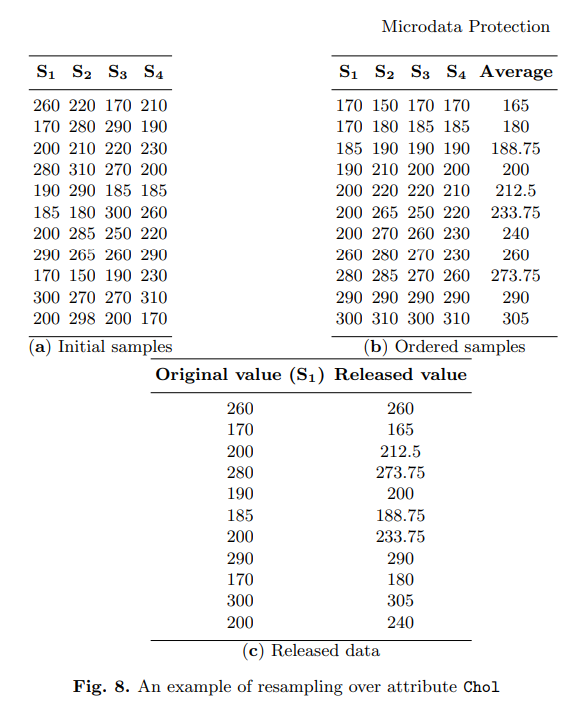
\includegraphics[width=0.5\linewidth]{paper_microdata/Fig8.png}
        \caption{Esempio di resampling}
        \label{fig:Fig-8}
    \end{figure}
    \item \textit{Rounding}: Simile alla tecnica usata anche per la protezione dei macrodati ed è applicabile solo agli attributi continui. Sostituisce i valori originali con dei valori approssimati, quest'ultimi sono scegli da un set di \textit{rounding points} $p_i$ ognuno il quale definisce il \textit{rounding set}. Per esempio: 
    \begin{itemize}
        \item \textit{\textbf{Rounding Points}} possono essere scelti come multipli di un valore base $b$, con $b = p_{i+1} - p_i$.
        \item \textit{\textbf{Rounding Sets}} definiti come 
        $\\$
        \begin{itemize}
            \item 
            $\begin{cases}
                [p_i - \frac{b}{2}, p_i + \frac{b}{2}) \text{con } i = 2,...,r-1 \\
                [0, p_1 + \frac{b}{2}) \\
                [p_r - \frac{b}{2}, X_{max}], \text{con } X_{max} \text{  il valore più grande possibile}
            \end{cases}$
            \item rispettivamente per $p_1$ e $p_r$
            \item Un valore $v$ di $X$ viene sostituito dal round point corrispondente al rounding set dove è contenuto $v$.
        \end{itemize}
    \end{itemize}
    
    \item \textit{Random Noise}: Perturba gli attributi sensibili aggiungendo o moltiplicando una variabile casuale con una distribuzione. Il rumore additivo (additive noise) è preferito al rumore moltiplicativo (multiplicative noise) e viene formalmente definito così:
    $\\$
   \textit{Poniamo $X_j$ come la $j_{esima}$ colonna della table dei microdati originaria corrispondente a un attributo sensibile e supponiamo che ci siano $N$ tuple.
    Ogni valore $X_{ij}$, con $i$ = $1,...,N$, viene sostituito con $x_{ij}$ + $\varepsilon_{ij}$, dove $\varepsilon_j$ è il vettore degli errori normalmente distribuiti ricavati da una variabile casuale con la media uguale a 0, in generale, con una varianza che sia proporzionale agli attributi originari}
    
    $\\$

    \textit{Forse da approfondire}
    
    \footnote{N.B $\epsilon$ viene usato per perturbare i dati ma lasciando intatta la correlazione con la tabella iniziale}
    
    \item \textit{Swapping}: Consiste nel modificare il subset di una table di microdati facendo lo swapping dei valori di un set formato degli attributi sensibili, chiamato \textit{swapped attributes}, tra coppie di tuple selezionate (le coppie sono selezionate secondo un criterio ben definito).
    Intuitivamente, questa tecnica riduce il rischio di re-identificazione perché introduce dell'incertezza sul valore reale legato al dato del respondent. Anche se questa tecnica è facile da applicare, generalmente ha lo svantaggio di non preservare le proprietà dei sottodomini. Inizialmente la tecnica originale fu presentata solamente per gli attributi categorici.
    
    \item \textit{Micro-Aggregation (o Blurring)}: Consiste nel raggupprare le tuple individiduali in piccole aggregazioni di una dimensione fissata $k$: verrà pubblicata la media di ogni aggregato invece dei valori individiduali. Anche se esistono diverse funzioni per caloclare la similrità, può essere difficile trovare un soluzione di raggruppamento ottimale. 
    Ci sono diverse varianti di \textit{micro-aggregation}, per esempio la media può sostituire il valore originale anche solo per una singola tupla nel gruppo o per tutte.
    Molti attributi possono essere protetti grazie a \textit{micro-aggregation} usando lo stesso o un diverso raggruppamento e, la dimensione del gruppo puo essere variabile o fissata ad un minimo. 
\end{itemize}
    
\section{Tecniche per la Generazione di Dati Sintetici}
La generazione dei dati sintetici è una valida alternaitiva per la protezione dei microdati. Il principio base su cui queste tecniche sono basate riguarda la non correlazione tra i contenuti statistici dei dati e l'informazione provvista da ogni respondent, quindi un modello ben rappresentante il dato potrebbe sostiture il dato stesso. Un requisito molto importante per la generazione dei dati sintetici, che rende il processo di generazione un problema importante, è che i dati sintetici e il dato originale potrebbero presentare la stessa qualità delle analisi statistiche. Il vantaggio maggiore di questi tipi di tecniche è che i dati sintetici rilasciati non sono collegati a nessun respondent, indi per cui il rilascio non può essere soggetto al fenomeno di re-identificazione; questo, inoltre, lascia ai proprietari dei dati di porre maggiore attenzione sulla qualità del dato rilasciato, invece che al problema di re-identificazione.

\section{Misure per valutare la confidenzialità e l'utilità dei Microdati}